% This file was created by tikzplotlib v0.9.8.
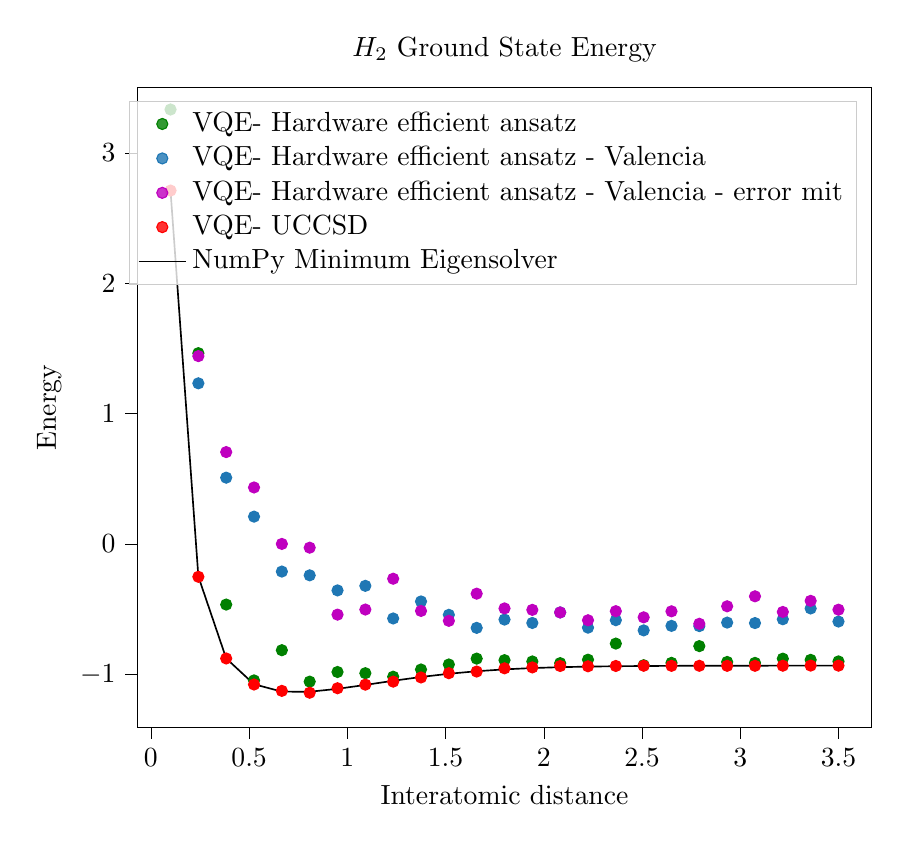
\begin{tikzpicture}

\definecolor{color0}{rgb}{0.12156862745098,0.466666666666667,0.705882352941177}
\definecolor{color1}{rgb}{1,1,1}
\definecolor{color2}{rgb}{0.75,0,0.75}

\begin{axis}[
width = 0.9\textwidth,
height = 0.8\textwidth,
legend cell align={left},
legend style={fill opacity=0.8, draw opacity=1, text opacity=1, draw=white!80!black},
tick align=outside,
tick pos=left,
title={\(\displaystyle H_2\) Ground State Energy},
x grid style={white!69.0196078431373!black},
xlabel={Interatomic distance},
xmin=-0.07, xmax=3.67,
xtick style={color=black},
y grid style={white!69.0196078431373!black},
ylabel={Energy},
ymin=-1.40511659547248, ymax=3.5,
ytick style={color=black}
]
\addplot [draw=green!50!black, fill=green!50!black, mark=*, only marks]
table{%
x  y
0.1 3.33404888388889
0.241666666666667 1.4645029490669
0.383333333333333 -0.46450550625885
0.525 -1.04651783607663
0.666666666666667 -0.814757346621391
0.808333333333333 -1.05595147241454
0.95 -0.981918023471895
1.09166666666667 -0.991141904256192
1.23333333333333 -1.01803695484038
1.375 -0.962856946671496
1.51666666666667 -0.924300954060679
1.65833333333333 -0.879327376496453
1.8 -0.891253988480295
1.94166666666667 -0.901161414081757
2.08333333333333 -0.913870958840689
2.225 -0.887565867606575
2.36666666666667 -0.763971778928865
2.50833333333333 -0.929820353754401
2.65 -0.911911751494509
2.79166666666667 -0.783467062591093
2.93333333333333 -0.904958407948391
3.075 -0.912188938998033
3.21666666666667 -0.879687740360926
3.35833333333333 -0.888788596051769
3.5 -0.900638903777969
};
\addlegendentry{VQE- Hardware efficient ansatz}
\addplot [draw=color0, fill=color0, mark=*, only marks]
table{%
x  y
0.1 4.13929602474146
0.241666666666667 1.23306214923331
0.383333333333333 0.509132360153934
0.525 0.210164137795337
0.666666666666667 -0.211311005144729
0.808333333333333 -0.24018451331369
0.95 -0.355852776989674
1.09166666666667 -0.320900619323827
1.23333333333333 -0.571274305064426
1.375 -0.440590850111626
1.51666666666667 -0.543331385415238
1.65833333333333 -0.643377178965285
1.8 -0.57987909525993
1.94166666666667 -0.605776984180282
2.08333333333333 -0.524944900771221
2.225 -0.641734614800259
2.36666666666667 -0.584436150920546
2.50833333333333 -0.662698462260614
2.65 -0.628147164954799
2.79166666666667 -0.629857081509611
2.93333333333333 -0.602913048395873
3.075 -0.606573997396377
3.21666666666667 -0.577190735466211
3.35833333333333 -0.494441927024351
3.5 -0.594889921846751
};
\addlegendentry{VQE- Hardware efficient ansatz - Valencia}
\addplot [draw=color2, fill=color2, mark=*, only marks]
table{%
x  y
0.1 3.90308358318452
0.241666666666667 1.44178771665008
0.383333333333333 0.705388462954166
0.525 0.433956897811221
0.666666666666667 0.000675256251612799
0.808333333333333 -0.0281592960288261
0.95 -0.541918976101957
1.09166666666667 -0.502787641777477
1.23333333333333 -0.26638027298495
1.375 -0.513405860192759
1.51666666666667 -0.589451633624822
1.65833333333333 -0.38101332326901
1.8 -0.494075925815565
1.94166666666667 -0.50524487674437
2.08333333333333 -0.525074078158373
2.225 -0.58503085709575
2.36666666666667 -0.515226320441291
2.50833333333333 -0.562513152085557
2.65 -0.51643111027973
2.79166666666667 -0.612088595274417
2.93333333333333 -0.477827624987215
3.075 -0.40123974815649
3.21666666666667 -0.5213009648001
3.35833333333333 -0.436078981943097
3.5 -0.503953854987049
};
\addlegendentry{VQE- Hardware efficient ansatz - Valencia - error mit}
\addplot [draw=red, fill=red, mark=*, only marks]
table{%
x  y
0.1 2.71198570072586
0.241666666666667 -0.251483195435701
0.383333333333333 -0.878173545869445
0.525 -1.07794644701999
0.666666666666667 -1.12683415579902
0.808333333333333 -1.14109694689087
0.95 -1.10664707155618
1.09166666666667 -1.07910627034727
1.23333333333333 -1.05592649073806
1.375 -1.02390479277029
1.51666666666667 -0.991188234776358
1.65833333333333 -0.978508783641437
1.8 -0.953791071541214
1.94166666666667 -0.946802432711941
2.08333333333333 -0.935957751848852
2.225 -0.938239597122296
2.36666666666667 -0.935708854721641
2.50833333333333 -0.934135184585209
2.65 -0.934653289723957
2.79166666666667 -0.934268141438297
2.93333333333333 -0.934654834036143
3.075 -0.934554805939235
3.21666666666667 -0.933677052075183
3.35833333333333 -0.932913452034017
3.5 -0.933358397132243
};
\addlegendentry{VQE- UCCSD}
\addplot [draw=black, semithick]
table {%
0.1 2.70996077086727
0.241666666666667 -0.249531837490203
0.383333333333333 -0.877883034274586
0.525 -1.07591365518925
0.666666666666667 -1.13270442393475
0.808333333333333 -1.1333543212074
0.95 -1.11133941773615
1.09166666666667 -1.08106467373544
1.23333333333333 -1.04940145259007
1.375 -1.020188902609
1.51666666666667 -0.995517295390776
1.65833333333333 -0.976135364799397
1.8 -0.961816952792584
1.94166666666667 -0.951768940753433
2.08333333333333 -0.945000304284272
2.225 -0.94057829412465
2.36666666666667 -0.937751505966631
2.50833333333333 -0.935971802698122
2.65 -0.934864128930254
2.79166666666667 -0.934181726507233
2.93333333333333 -0.933765772436944
3.075 -0.933515219985053
3.21666666666667 -0.933366258704161
3.35833333333333 -0.933278912315146
3.5 -0.933228405549716
};
\addlegendentry{NumPy Minimum Eigensolver}
\end{axis}

\end{tikzpicture}
